\section{Beam Modelling with Measurements of Galactic HI}
\label{sec:beam_model}

The Hydrogen I (HI) emission line is an omnipresent and easily identifiable time-varying signal within the GReX observing band, making it an ideal metric for ensuring that a GReX terminal is observing the sky properly. 
Captured spectra in the \textit{Prometheus} database are accessed by Grafana to display estimates of the HI SNR in real time at the top of all Grafana dashboard monitors. 
While the HI-line intensity provides a useful sanity check that a terminal is properly observing the sky, its usefulness does not end there.
In this section, we present the results of our method for using the measured HI-line intensity at the OVRO and Cornell terminals to estimate the FWHM (and corresponding solid angle) of the GReX antenna beam-response.

Following the prescription detailed in \autoref{sec:Asimulation}, we use the Leiden/Argentine/Bohn (LAB) all-sky survey of galactic neutral hydrogen~\cite{kalberlaLeidenArgentineBonn2005} to simulate the expected antenna temperature as seen by the terminal over one sidereal day (sampled every 10 minutes) for fifty different beams with $\theta_\text{FWHM}$s ranging from $50^\circ$ to $100^\circ$. 
We query HI-line observations from the Cornell and OVRO \textit{Prometheus} databases with time steps of ten minutes over a month. 
We only keep days where the data is continuous across the day to consistently align the data and simulations according to the local sidereal time (LST) before normalizing both such that the average temperature over one day is a constant between all simulations and observations. 
For each time sample across the sidereal day, we calculate the observed HI-line mean intensity and standard deviation. 
Any samples that exceed a $3\sigma$ deviation from the mean are considered to be impacted by RFI and are ignored when calculating the root-mean squared (RMS) residuals between observations and models. 
Any days with more than 5\% of samples above this threshold are fully ignored. 
After RFI mitigation, there are 23 and 11 days remaining from the Cornell and OVRO measurements, respectively. 
With the data aligned, normalized, and cleaned of RFI, we calculate the RMS error between each day and each model. 
\autoref{fig:HIsimFit} presents the aligned and normalized observed and simulated HI-line (left) alongside the RMS errors of each day against all modeled beam-shapes (right).
While all RMS curves display consistent profiles which have minima that are clustered around the average FWHM, there are some curves in \autoref{fig:HIsimFit} \textbf{(d)} that minimize at a higher RMS than is typical. 
We attribute this to the presence of RFI-affected samples that did not get removed by our thresholding process.
The modeled $\theta_\text{FWHM}$s corresponding to the RMS minimum for each day are taken as the population of best-fit parameters. 
We determine the general best fit model as the mean of this population, with a $1\sigma$ uncertainty in the FWHM given by the population standard deviation. 
Using this method, we determine that the Cornell terminal has a beam response at $1420.4\,\text{MHz}$ that is well-characterized as a 2D Gaussian with $\theta_\text{FWHM}^\text{CU}(1420.4\,\text{MHz})=67.44^\circ\pm0.99^\circ$. 
The OVRO terminal is similarly described by a $\theta_\text{FWHM}^\text{OVRO}(1420.4\,\text{MHz})=64.29^\circ\pm0.62^\circ$. 

\begin{figure}[ht!]
    \centering    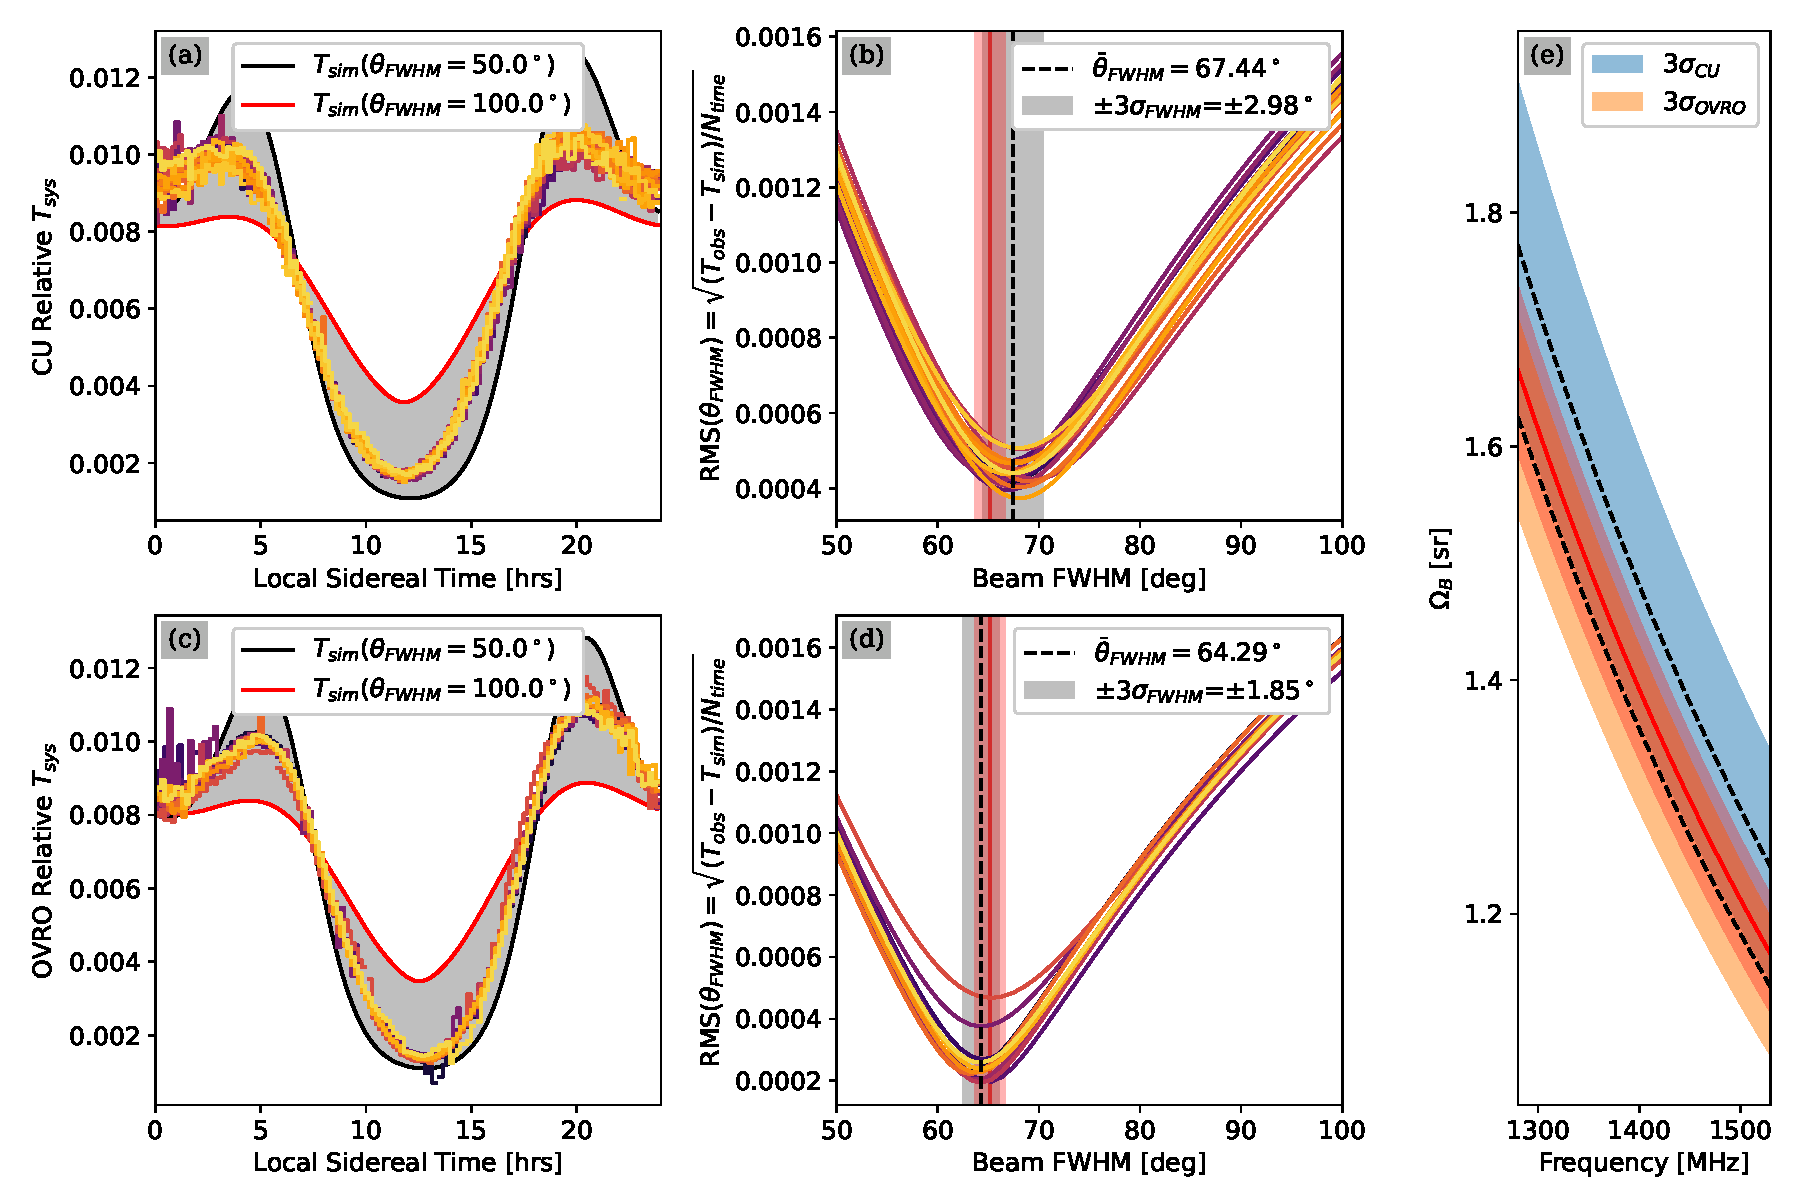
\includegraphics[width=1.0\textwidth]{figures/HIsimFit.pdf}
    \caption[HI observation-based GReX beam modelling]{Observed data and corresponding simulations of the HI-line by the OVRO (\textbf{(a)} and \textbf{(b)}) and Cornell (\textbf{(c)} and \textbf{(d)}) GReX terminals are used to fit the beam FWHM at 1420.4MHz. Simulations are rendered following the prescription in \autoref{sec:Asimulation}. The observed (colored step-function lines) and simulated data (gray shaded region bounded by red and black curves) are aligned by local sidereal time and samples overly affected by RFI are excluded when calculating the RMS error. The population of FWHM values that minimize the RMS errors for each terminal and each day are then used to determine the mean (black dashed line, \textbf{(b)} and \textbf{(d)}) and standard deviation of each terminal FWHM. The characteristic FWHM of a GReX terminal (\autoref{eq:popFWHM}) is presented in \textbf{(b)} and \textbf{(d)} as a solid red line with $3\sigma$ shading. We then scale the solid angle across the observing band according to the relationship $\Omega_B\propto f^{-2}$ in \textbf{(e)}.}\label{fig:HIsimFit}
\end{figure}

Since all GReX terminals are outfitted with identical feeds, we consider the beam response of a typical feed to be a good description for all feeds. 
This typical beam response at $1420.4\,\text{MHz}$ is then characterized as
\begin{equation}
    \theta_\text{FWHM} = \frac{\frac{\theta_\text{FWHM}^\text{OVRO}}{\sigma_\text{OVRO}^2}+\frac{\theta_\text{FWHM}^\text{CU}}{\sigma_\text{CU}^2}}{\frac{1}{\sigma_\text{OVRO}^2}+\frac{1}{\sigma_\text{CU}^2}}\pm\sqrt{\frac{1}{\frac{1}{\sigma_\text{OVRO}^2}+\frac{1}{\sigma_\text{CU}^2}}}=65.18^\circ\pm0.53\label{eq:popFWHM}
\end{equation}
with corresponding solid angle at that frequency of \begin{equation}
    \Omega_B=\int_\Omega d\Omega \exp{\left[-4\ln2\left(\frac{\theta}{\theta_\text{FWHM}}\right)^2\right]}= 1.36\,\pm0.02\,\text{sr}.
    \label{eq:beam_solid_angle}
\end{equation}
We use $\Omega_B\propto f^{-2}$ to determine the solid angle as a function of frequency,
\begin{equation}
\Omega_B(f)=\frac{1931.7\pm28.4}{f^2} \,\text{sr}\,\text{MHz}^2.
\end{equation}
This functional relationship (and equivalent comparisons for the individual terminal fits) is presented in \autoref{fig:HIsimFit} (\textbf{e}). 
We determine from this relation that the beam solid angle near our central frequency is $\Omega_B(1400\,\text{MHz})=1.40\,\pm0.02\,\text{sr}$. 
We also report the maximum effective area $A_0$ of the receiver across the band as $A_0=328\,\pm5\,\text{cm}^2$ according to \autoref{eq:Ae}. 
